\section{Evaluation Results}

\subsection{Evaluation Setup}
To comprehensively evaluate different models throughout the scientific discovery workflow, we performed quantitative assessments across diverse LLMs and agents using scientist-aligned metrics.
\begin{itemize}
    \item For open-weight LLMs, we evaluated DeepSeek-V3.2~\cite{DeepSeekV3.2_2025}, DeepSeek-R1~\cite{Guo2025}, Intern-S1 and Intern-S1-mini~\cite{bai2025intern}, Kimi-k2~\cite{team2025kimi}, Qwen3-VL-235B-A22B~\cite{bai2025qwen3}, Qwen3-235B-A22B, Qwen3-Max, and Qwen3-8B~\cite{yang2025qwen3}, and Llama-4-Scout~\cite{Llama4_Release2025}.
    \item For closed-weight LLMs, we assessed GPT-4o~\cite{GPT4o_SystemCard2024}, GPT-4.1~\cite{GPT4.1_Docs2025}, GPT-5~\cite{GPT5_SystemCard2025}, GPT-5.1~\cite{GPT5.1_Addendum2025}, o3 and o4-mini~\cite{OpenAI_o3_2025}, Gemini-2.5-Flash and Gemini-2.5-Pro~\cite{comanici2025gemini}, Gemini-3-Pro~\cite{Gemini3_DeepMind2025}, Claude-Opus-4.1~\cite{ClaudeOpus4.1_2025}, Claude-Sonnet-4.5~\cite{ClaudeSonnet4.5_2025}, Grok-3~\cite{Grok3_2025}, and Grok-4~\cite{Grok4_ModelCard2025}.
    \item For open-source agents, we tested SmolAgents(GPT-4.1) and SmolAgents(Gemini-2.5-Flash)~\cite{SmolAgents_2025}, Owl(GPT-4.1) and Owl(Gemini-2.5-Flash)~\cite{hu2025owl}, WebThinker~\cite{WebThinker_NeurIPS2025}, XMaster~\cite{XMaster_Arxiv2025}, and InternAgent~\cite{team2025novelseek}.
    \item For closed-source agents, we evaluated OpenAI Deep Research(o3) and OpenAI Deep Research(o4-mini)~\cite{DeepResearch_OpenAI2025}, Kimi-Search(Kimi-k2)~\cite{KimiResearcher_2025}, Doubao-Search(Seed-1-6), Grok-Search(Grok-4)~\cite{GrokDeepSearch_2025}, and Perplexity(Sonar-Pro)~\cite{Perplexity_DeepResearch_2025}.
\end{itemize}
For benchmarking consistency, we set the temperature of all configurable models to 0 to minimize randomness and used a standard zero-shot, task-specific prompt template across all tasks.


\subsection{Overview}

Table~\ref{tab:llm_comparison} provides a cross‑task snapshot of current capabilities. Overall, SGI‑Score remains low across families (typically ~30±5), with the best aggregate result at 33.83 (Gemini‑3‑Pro). Closed‑source models show only a marginal edge over leading open‑source systems (e.g., Claude‑Sonnet‑4.5 at 32.16 vs. Qwen3‑Max at 31.97), indicating that scale and access alone do not translate into robust scientific cognition. At the task level, Deep Research is the most brittle under the strict Exact‑Match metric (best 18.48; many models around 8–16), revealing the difficulty of end‑to‑end, multi‑source evidence integration and numerically faithful inference. Idea Generation exhibits the opposite pattern—strong surface performance but weak realizability: while GPT‑5 attains the highest average (55.40), feasibility remains uniformly low across models, reflecting underspecified implementation details and missing resource/parameter assumptions. In Dry Experiments, high executability does not imply correctness: even the best PassAll@5 peaks at 36.64 (Gemini‑3‑Pro), underscoring persistent gaps in numerical stability and scientific algorithm selection. Wet Experiments remain challenging, with uniformly low action‑sequence similarity and only moderate parameter accuracy, driven by errors in step ordering, temporal coordination, and branch/sample bookkeeping. Multimodal Experimental Reasoning shows relatively stronger results (best MCA 41.92), yet remains far from reliable scientific discrimination. Taken together, these patterns validate our SGI framing: contemporary models possess fragments of the Deliberation–Conception–Action–Perception cycle but fail to integrate them into a coherent, workflow‑faithful intelligence—pointing to the need for meta‑analytic retrieval with numerical rigor, planning‑aware conception, and procedure‑level consistency constraints.

\begin{table}[t]
\centering
\renewcommand{\arraystretch}{0.9}
\setlength{\tabcolsep}{2pt}
\tiny
\resizebox{15cm}{!}{
\begin{tabular}{lccccc c}
\toprule
\rowcolor{yellow!50}\textbf{Model} & \textbf{DeepResearch} & \textbf{IdeaGen} & \textbf{DryExp} & \textbf{WetExp} & \textbf{ExpReasoning} & \textbf{SGI-Score} \\
\midrule

\rowcolor{blue!5}\multicolumn{7}{c}{\emph{Open-source LLM}} \\ \arrayrulecolor{black!30}\midrule
DeepSeek-V3.2 & 12.70 & 37.45 & 23.62 & 20.95 & - & \cellcolor{red!10}- \\
DeepSeek-R1 & 15.03 & 40.16 & 33.33 & 21.12 & - & \cellcolor{red!10}- \\
Intern-S1 & 15.74 & 38.09 & 28.79 & 29.02 & 28.87 & \cellcolor{red!10}28.10 \\
Intern-S1-mini & 11.06 & 36.04 & 16.97 & 12.42 & 16.84 & \cellcolor{red!10}18.67 \\
Kimi-k2 & 13.11 & 43.17 & 29.52 & 25.76 & - & \cellcolor{red!10}- \\
Qwen3-VL-235B-A22B & 11.97 & 39.28 & 28.41 & 30.30 & 31.62 & \cellcolor{red!10}28.32 \\
Qwen3-235B-A22B & 14.19 & 39.45 & 28.89 & 26.40 & - & \cellcolor{red!10}- \\
Qwen3-Max & 15.38 & 39.83 & 33.21 & 33.62 & 37.80$^{*}$ & \cellcolor{red!10}31.97$^{*}$\copper \\
Qwen3-8B & 8.18 & 35.78 & 18.45 & 9.96 & 23.37$^{*}$ & \cellcolor{red!10}19.15$^{*}$ \\
Llama-4-Scout & 7.86 & 29.72 & 20.37 & 21.66 & 25.77 & \cellcolor{red!10}21.08 \\
\arrayrulecolor{black!100}\midrule

\rowcolor{blue!5}\multicolumn{7}{c}{\emph{Closed-source LLM}} \\ \arrayrulecolor{black!30}\midrule
GPT-4o & 7.86 & 35.95 & 26.94 & 31.31 & 32.30 & \cellcolor{red!10}26.87 \\
GPT-4.1 & 11.32 & 36.49 & 34.32 & 36.63 & 38.49 & \cellcolor{red!10}31.45 \\
GPT-5 & 14.47 & \cellcolor{blue!10}\textbf{55.40} & 29.89 & 16.31 & 38.14 & \cellcolor{red!10}30.84 \\
GPT-5.1 & 11.64 & 47.12 & 31.00 & 22.77 & 34.02 & \cellcolor{red!10}29.31 \\
o3 & 12.89 & 46.07 & 31.73 & 30.04 & 32.65 & \cellcolor{red!10}30.68 \\
o4-mini & 11.95 & 40.78 & 35.79 & 28.86 & 33.33 & \cellcolor{red!10}30.14 \\
Gemini-2.5-Flash & 10.69 & 39.13 & 21.03 & 18.55 & 34.36 & \cellcolor{red!10}24.75 \\
Gemini-2.5-Pro & 15.09 & 39.95 & 22.51 & 22.05 & 41.24 & \cellcolor{red!10}28.17 \\
Gemini-3-Pro & \cellcolor{blue!10}\textbf{18.48} & 39.68 & \cellcolor{blue!10}\textbf{36.64} & 32.45 & \cellcolor{blue!10}\textbf{41.92} & \cellcolor{red!10}\textbf{33.83}\gold  \\
Claude-Opus-4.1 & 12.93 & 40.29 & 34.69 & 25.38 & 38.83 & \cellcolor{red!10}30.42 \\
Claude-Sonnet-4.5 & 13.84 & 43.20 & 35.79 & 30.15 & 37.80 & \cellcolor{red!10}32.16\silver \\
Grok-3 & 13.52 & 35.98 & 27.31 & \cellcolor{blue!10}\textbf{37.92} & - & \cellcolor{red!10}- \\
Grok-4 & 13.31 & 37.12 & 33.71 & 29.01 & 30.24 & \cellcolor{red!10}28.68 \\
\arrayrulecolor{black!100}\bottomrule
\end{tabular}
}
\caption{\textbf{Overview Results Across SGI-Bench Tasks}: Aggregated performance across Deep Research, Idea Generation, Dry/Wet Experiment, and Scientific Experimental Reasoning. The scores for Deep Research are based on the exact match metric (the strictest metric). Idea Generation scores are the average of four metrics evaluating ideas. Dry Experiment scores are based on PassAll@5 (the strictest metric). Wet Experiment scores are the average of action sequence similarity and parameter accuracy. Experimental Reasoning scores are based on the multi-choice accuracy metric (the strictest metric). The SGI-Score is the average across these tasks, reflecting the overall capability of an AI model in various scientific research scenarios. An asterisk $^{*}$ indicates results from different versions of the same series of multimodal models.}
\label{tab:llm_comparison}
\end{table}



\subsection{Scientific Deep Research}

\begin{figure}[ht]
% \vspace{-0.5em}
\centerline
{\includegraphics[width=16cm]{paper/imgs/deepresearch_case1.png}}
\caption{\textbf{Scientific Deep Research Case}: Example multi-hop workflow illustrating data retrieval, evidence synthesis, and quantitative analysis.}
\label{fig: search_case1}
% \vspace{-2em}
\end{figure}


The results for LLMs and agents are presented in Figs.~\ref{fig: llms deep research} and~\ref{fig: agents deep research}. Exact Match (EM) evaluates the correctness of the final answer, while Step-Level Accuracy (SLA) measures alignment with the reference reasoning trajectory. EM remains low across all evaluated systems, typically around 10\% and seldom above 20\%, indicating that current models capture only a narrow fraction of the analytical depth required for scientific deep research. While top-performing tool-augmented agents slightly outperform the best offline LLMs on SLA, the overall distributions overlap substantially; several agent systems underperform many LLMs, and EM differences are marginal with the best LLMs matching or exceeding the best agents.

\textbf{SLA substantially exceeds EM across nearly all systems.}
Multiple systems, including several agents—achieve SLA above 50\%, with the best around 65\%. This disparity suggests that models frequently produce partially correct or locally consistent reasoning steps but struggle to maintain coherence and correctness across the full reasoning chain. Such behavior underscores the intrinsic difficulty of end-to-end scientific reasoning and the importance of step-wise decomposition for improving task success.

\textbf{Newer large-scale LLMs do not universally outperform predecessor models. }
For example, Grok-4 exhibits lower EM and SLA than Grok-3 on this benchmark, suggesting that large-scale training may introduce regressions or reduce retention of specialized scientific knowledge. These results collectively highlight the current limitations of frontier AI systems in executing the multi-faceted and rigorously structured reasoning processes required for Scientific Deep Research.

\begin{figure}[ht]
% \vspace{-0.5em}
\centerline
{\includegraphics[width=17cm]{paper/imgs/LLMs_deep_research_metrics.png}}
\caption{\textbf{Scientific Deep Research Evaluation of LLMs}: Exact Match (EM) and Step-Level Accuracy (SLA) across models using scientist-aligned metrics.}
\label{fig: llms deep research}
% \vspace{-2em}
\end{figure}

\begin{figure}[ht]
% \vspace{-0.5em}
\centerline
{\includegraphics[width=17cm]{paper/imgs/Agents_deep_research_metrics.png}}
\caption{\textbf{Scientific Deep Research Evaluation of Multi-Agent Systems}: EM and SLA for tool-augmented agent systems.}
\label{fig: agents deep research}
% \vspace{-2em}
\end{figure}


\begin{figure}[ht]
% \vspace{-0.5em}
\centerline
{\includegraphics[width=17cm]{paper/imgs/LLMs_Agents_task_metric.png}}
\caption{\textbf{Scientific Deep Research Performance by Type}: Comparison across Data, Properties, Micro-Experiments, and Macro-Experiments categories.}
\label{fig: deep research on different task}
% \vspace{-2em}
\end{figure}

\textbf{Most models exhibit substantially lower performance on the Data and Properties tasks, but somewhat better—though still modestly—on Micro- and Macro-experiment tasks.}
Based on the focus of each question, we categorize the tasks into four types: Data, Properties, Micro-experiments, and Macro-experiments (Table~\ref{tab:deep_research_types}). Figure~\ref{fig: deep research on different task} summarizes the performance of LLMs and agents across these categories. Notably, performance across all four categories rarely exceeds 30\% (with only a few Macro cases slightly above), underscoring the intrinsic difficulty of scientific deep research. This disparity can be attributed to the nature of the information required. Data- and property-related questions often rely on detailed numerical specifications or contextual descriptions scattered across disparate sources in the literature, demanding precise retrieval, cross-referencing, and aggregation. In contrast, Micro- and Macro-experiment tasks tend to provide more structured protocols or clearer experimental outcomes, enabling LLMs and agents to reason with fewer retrieval uncertainties.

In summary, the relatively stronger model performance on experiment-oriented tasks suggests that recent advances in LLM pretraining and instruction tuning have enhanced models’ abilities to process structured procedures and numerical patterns. Nevertheless, the consistently low scores across all categories indicate that contemporary LLMs, even when augmented with tool-based agents, remain far from mastering the breadth and depth of reasoning required for robust scientific deep research.


\subsection{Idea Generation}


\begin{figure}[ht]
% \vspace{-0.5em}
\centerline
{\includegraphics[width=17cm]{paper/imgs/idea_case.png}}
\caption{\textbf{Idea Generation Case}: Input information such as related work and objective, and output a structured idea, including a graph consisting of specific implementation steps.}
\label{fig: idea_case}
% \vspace{-2em}
\end{figure}


\begin{table}[t]
\centering
\renewcommand{\arraystretch}{0.9}
\setlength{\tabcolsep}{2pt}
\tiny
\resizebox{13cm}{!}{
\begin{tabular}{lccccc}
\toprule
\textbf{Model} & \textbf{Effectiveness} & \textbf{Novelty} & \textbf{Detailedness} & \textbf{Feasibility}  & \textbf{Average} \\
\midrule

\rowcolor{blue!5}\multicolumn{6}{c}{\emph{Open-source LLM}} \\ \arrayrulecolor{black!30}\midrule
DeepSeek-V3.2 & 28.09 & 54.09 & 47.34 & 20.28 & 37.45 \\
DeepSeek-R1 & 27.73 & 63.64 & 50.06 & 19.20 & 40.16 \\
Intern-S1 & 26.38 & 56.47 & 49.10 & 20.42 & 38.09 \\
Intern-S1-mini & 24.95 & 55.71 & 48.07 & 15.44 & 36.04 \\
Kimi-k2 & 25.24 & 69.49 & 59.20 & 18.74 & 43.17 \\
Qwen3-VL-235B-A22B & 27.24 & 59.53 & 50.23 & 20.14 & 39.28 \\
Qwen3-235B-A22B & 26.63 & 62.05 & 49.73 & 19.40 & 39.45 \\
Qwen3-Max & 28.74 & 59.01 & 50.61 & 20.98 & 39.83 \\
Qwen3-8B & 26.12 & 49.36 & 47.09 & 20.58 & 35.78 \\
Llama-4-Scout & 28.50 & 33.25 & 43.08 & 14.06 & 29.72 \\
\arrayrulecolor{black!100}\midrule

\rowcolor{blue!5}\multicolumn{6}{c}{\emph{Closed-source LLM}} \\ \arrayrulecolor{black!30}\midrule
GPT-4o & 27.28 & 48.19 & 47.85 & 20.51 & 35.95 \\
GPT-4.1 & 27.49 & 48.72 & 47.88 & 21.87 & 36.49 \\
GPT-5 & \cellcolor{blue!10}\textbf{40.92} & \cellcolor{blue!10}\textbf{76.08} & \cellcolor{blue!10}\textbf{85.72} & 18.87 & \cellcolor{blue!10}\textbf{55.40} \\
GPT-5.1 & 36.07 & 66.98 & 66.62 & 18.83 & 47.12 \\
o3 & 29.42 & 73.74 & 58.22 & \cellcolor{blue!10}\textbf{22.90} & 46.07 \\
o4-mini & 27.26 & 63.33 & 50.53 & 22.01 & 40.78 \\
Gemini-2.5-Flash & 28.45 & 56.91 & 50.49 & 20.69 & 39.13 \\
Gemini-2.5-Pro & 30.98 & 57.54 & 52.21 & 19.06 & 39.95 \\
Gemini-3-Pro & 28.38 & 59.41 & 51.07 & 19.87 & 39.68 \\
Claude-Opus-4.1 & 26.52 & 64.40 & 50.16 & 20.07 & 40.29 \\
Claude-Sonnet-4.5 & 32.01 & 58.00 & 61.75 & 21.03 & 43.20 \\
Grok-3 & 28.37 & 46.27 & 48.35 & 20.93 & 35.98 \\
Grok-4 & 28.46 & 50.93 & 49.48 & 19.60 & 37.12 \\
\arrayrulecolor{black!100}\bottomrule
\end{tabular}
}
\caption{\textbf{Idea Generation Results}: The ideas generated by the model outperformed the average proportion of the original papers in the four dimensions of Effectiveness, Novelty, Detailedness, and Feasibility.}
\label{tab:idea_gen_res}
\end{table}

Figure~\ref{fig: idea_case} illustrates the evaluation pipeline for Idea Generation in SGI-Bench, and more experimental details can be found in the section~\ref{Metrics: Idea Gen}. Table~\ref{tab:idea_gen_res} shows the quantitative experimental results of idea generation, including effectiveness, novelty, detailedness, and feasibility. We could see that GPT-5 achieves the best average performance, and achieves the best performance in three aspects only excluding the feasibility. Moreover, across models, a clear pattern emerges: Novelty is generally high, especially among closed-source systems (e.g., o3 73.74, GPT-5 76.08). This indicates that modern LLMs possess a robust capacity for generating conceptually novel scientific ideas. Such behavior aligns with the growing empirical use of LLMs as inspiration engines for scientific hypothesis generation and exploratory research. 


Mechanistically, this strength likely stems from their broad pretraining over heterogeneous scientific corpora, which enables them to recombine distant concepts across domains, as well as their ability to internalize high-level research patterns (problem--method--evaluation triples). 
As a result, LLMs are particularly effective at proposing \emph{plausible and novel conceptual directions}, often exceeding what a single human researcher can enumerate in a short time window.


\textbf{Novelty is relatively high while feasibility lags.}
In contrast, Effectiveness is modest for most models and Feasibility consistently lags behind the other dimensions. Even the best-performing GPT-5, which achieves high Detailedness (85.72) and the highest Average (55.40), attains only scores 18.87 in Feasibility, confirming that conceptual richness does not reliably translate into implementation-ready plans. The top Feasibility model by our metric is o3 (22.90), while open-source feasibility peaks at Qwen3-8B (20.58); other models cluster in the 14–20 range. Open-source models exhibit the same trend: Kimi-k2 reaches higher Detailedness (59.20) but remains limited in Feasibility (18.74); similarly, Qwen3-VL-235B-A22B reaches only 20.14 in Feasibility despite substantially higher conceptual elaboration (50.23).

\textbf{Execution details are often underspecified.}
These outcomes reveal a realization bottleneck in current idea generation: While models can articulate sophisticated pipelines at a high level, they frequently omit or under-specify key executable details. Typical failure issues include: (i) data references without acquisition or preprocessing plans; (ii) training and optimization loops that omit concrete hyperparameters or resource assumptions; (iii) algorithmic modules named but not grounded in precise choices (e.g., solver type, training objective, evaluation protocol); (iv) integration steps that fail to specify interfaces, ordering, or data flow. Consequently, many proposals fail feasibility checks not because they are conceptually unsound, but because they rely on implicit, unparameterized execution assumptions that cannot be validated under realistic experimental conditions. 
This gap highlights a fundamental limitation of current LLMs: they excel at linguistic and conceptual abstraction, yet struggle with the procedural, resource-aware, and constraint-grounded planning required for real scientific implementation. 

Overall, the Idea Generation results indicate that contemporary LLMs are adept at proposing novel directions but struggle to turn them into fully executable plans. Bridging this gap will require constraint-aware planning, stronger priors over experimental and engineering practice, tool-augmented verification (e.g., property simulators, data/API discovery, and reproducibility scaffolds), and training signals that reward concrete, parameterized, and testable implementation steps rather than stylistic innovation.



\subsection{AI-Assisted Scientific Experiment}

Experiments form the critical bridge between idea generation and scientific reasoning, providing the most direct avenue for validating hypotheses and uncovering new phenomena. Within SGI-Bench, we evaluate two complementary forms of experiments: \emph{dry experiments}, which involve computational analyses or simulations, and \emph{wet experiments}, which require laboratory procedures and operational planning. Across both categories, current AI models exhibit substantial limitations, revealing a persistent gap between linguistic fluency and experimentally actionable competence.

\subsubsection{Dry Experiment}

\begin{figure}[ht]
% \vspace{-0.5em}
\centerline
{\includegraphics[width=16cm]{paper/imgs/code_case1.png}}
\caption{\textbf{Dry Experiment Code Examples}: Masked-function completion setup with I/O formats, and functional descriptions.}
\label{fig: code_case1}
% \vspace{-2em}
\end{figure}

As introduced in Section~\ref{sec: Task Definition of Experiment}, each dry experiment contains three components: a description of scientific background, a complete data-construction script, and an analysis script with masked functions. The model must infer and complete these missing functions using contextual understanding. For fairness and structural clarity, function headers, including names, signatures, and functional descriptions, are preserved, as shown in Figure~\ref{fig: code_case1}. This setup isolates the model’s ability to infer algorithmic logic rather than boilerplate structure.


\begin{table}[t]
\centering
\renewcommand{\arraystretch}{0.9}
\setlength{\tabcolsep}{2pt}
\tiny
\resizebox{14cm}{!}{
\begin{tabular}{lccccc}
\toprule
\textbf{Model} & \textbf{PassAll@5(\%)$\uparrow$} & \textbf{PassAll@3(\%)$\uparrow$} & \textbf{PassAll@1(\%)$\uparrow$} & \textbf{AET(s)$\downarrow$} & \textbf{SER(\%)$\uparrow$} \\
\midrule

\rowcolor{blue!5}\multicolumn{6}{c}{\emph{Open-source LLM}} \\ \arrayrulecolor{black!30}\midrule
DeepSeek-V3.2 & 23.62 & 26.94 & 29.52 & 29.96 & 68.27 \\
DeepSeek-R1 & 33.33 & 35.56 & 37.41 & 28.09 & 91.70 \\
Intern-S1 & 28.79 & 31.44 & 34.09 & 31.04 & 87.58 \\
Intern-S1-mini & 16.97 & 17.34 & 18.08 & 14.55 & 79.83 \\
Kimi-k2 & 29.52 & 32.10 & 36.16 & 33.42 & 90.26 \\
Qwen3-VL-235B-A22B & 28.41 & 31.37 & 33.58 & 32.74 & 91.22 \\
Qwen3-235B-A22B & 28.89 & 31.48 & 34.44 & 30.68 & 90.81 \\
Qwen3-Max & 33.21 & 35.42 & 37.27 & 35.25 & 90.33 \\
Qwen3-8B & 18.45 & 20.30 & 21.03 & 21.13 & 71.51 \\
Llama-4-Scout & 20.37 & 21.48 & 22.59 & 24.24 & 68.52 \\
\arrayrulecolor{black!100}\midrule

\rowcolor{blue!5}\multicolumn{6}{c}{\emph{Closed-source LLM}} \\ \arrayrulecolor{black!30}\midrule
GPT-4o & 26.94 & 29.89 & 32.10 & 37.90 & 79.78 \\
GPT-4.1 & 34.32 & 37.64 & 40.22 & 40.54 & 94.10 \\
GPT-5 & 29.89 & 32.84 & 34.69 & 34.54 & 75.50 \\
GPT-5.1 & 31.00 & 35.42 & 38.01 & 23.87 & 96.53 \\
o3 & 31.73 & 34.32 & 37.64 & 34.06 & 85.17 \\
o4-mini & 35.79 & 39.11 & 41.70 & 31.34 & 87.60 \\
Gemini-2.5-Flash & 21.03 & 22.51 & 24.72 & 15.09 & 44.65 \\
Gemini-2.5-Pro & 22.51 & 23.99 & 24.72 & \cellcolor{blue!10}\textbf{13.94} & 44.65 \\
Gemini-3-Pro & \cellcolor{blue!10}\textbf{36.64} & \cellcolor{blue!10}\textbf{40.46} & 41.98 & 21.16 & \cellcolor{blue!10}\textbf{98.85} \\
Claude-Opus-4.1 & 34.69 & 37.27 & 40.59 & 31.67 & 94.32 \\
Claude-Sonnet-4.5 & 35.79 & 38.75 & \cellcolor{blue!10}\textbf{42.07} & 31.59 & 94.83 \\
Grok-3 & 27.31 & 29.15 & 32.10 & 35.30 & 91.22 \\
Grok-4 & 33.71 & 37.12 & 40.53 & 33.74 & 94.09 \\

\arrayrulecolor{black!100}\bottomrule
\end{tabular}
}
\caption{\textbf{Dry Experiment Metrics Across Models}: PassAll@k, Average Execution Time (AET), and Smooth Execution Rate (SER) under five unit tests per problem.}
\label{tab:code metrics}
\end{table}

Table~\ref{tab:code metrics} summarizes three metrics defined in Section~\ref{sec: Metric of Dry Experiment}: \textit{PassAll@k}, \textit{Average Execution Time (AET)}, and \textit{Smooth Execution Rate (SER)}. Here, PassAll@k denotes passing at least $k$ out of five unit tests per problem. Under the lenient criterion ($k{=}1$), the best models achieve a \textit{PassAll@1} score of 42.07\%, whereas the strictest requirement ($k{=}5$) reduces performance to 36.64\%. These results underscore that scientific code completion remains a significant bottleneck, even for frontier LLMs. Notably, closed-source models generally achieve higher PassAll@k than leading open-source models, though the advantage is modest and distributions overlap, suggesting that scientific code synthesis in dry experiments remains underdeveloped across architectures.

\textbf{High execution rates do not guarantee correctness.}
The \textit{SER} metric captures whether the generated code executes without error, independent of correctness. While many top models achieve high SER values (>90\%), performance varies widely across systems; several models are substantially below this threshold (e.g., Gemini-2.5-Flash/Pro, Qwen3-8B, Llama-4-Scout, GPT-5, GPT-4o), indicating nontrivial robustness gaps. This suggests that basic structural and API-level reasoning has matured for some models; however, the persistent gap between \textit{SER} and accuracy metrics highlights that structural validity is far easier than algorithmic correctness in scientific contexts.


\begin{figure}[ht]
% \vspace{-0.5em}
\centerline
{\includegraphics[width=16cm]{paper/imgs/dry_task_metric.png}}
\caption{\textbf{PassAll@5 by Function Category}: Completion accuracy across numerical calculation, statistical analysis, simulation, metric calculation, data processing, and predictive modeling.}
\label{fig: dry_task_metric}
% \vspace{-2em}
\end{figure}

\textbf{Numerical and simulation functions are the most challenging.}
Figure~\ref{fig: dry_task_metric} breaks down \textit{PassAll@5} across functional types. Models perform relatively well on \textit{Data Processing} and \textit{Predictive Modeling}, where multiple valid implementations exist and errors are less amplified. In contrast, \textit{Numerical Calculation} and simulation-oriented functions prove substantially more difficult. These tasks typically require precise numerical stability, accurate discretization, or careful handling of domain-specific constraints, all of which amplify small reasoning inconsistencies. This pattern reveals a striking asymmetry: models exhibit reasonable flexibility in tasks with diverse valid outputs but struggle with tasks requiring exact numerical fidelity.


\begin{figure}[ht]
% \vspace{-0.5em}
\centerline
{\includegraphics[width=16cm]{paper/imgs/code_case2.png}}
\caption{\textbf{Dry Experiment Case Study}: Gravitational-wave computation highlighting the impact of numerical integration strategy on scientific outcomes.}
\label{fig: code_case2}
% \vspace{-2em}
\end{figure}

\textbf{Methodological choices critically affect outcomes.}
The case shown in Figure~\ref{fig: code_case2} illustrates this issue in an astronomical dry experiment involving the computation of gravitational-wave observables from LIGO/Virgo–like detectors. The o4-mini model employs a naïve numerical integration via \texttt{np.cumsum}, effectively using a forward Euler approximation for 
\[
\chi(z) = \int_0^z \frac{d\chi}{dz} dz,
\]
which introduces substantial cumulative error when the discretization is coarse. In contrast, GPT-4.1 correctly adopts \texttt{scipy.integrate.quad}, leveraging adaptive integration schemes that preserve numerical precision. Because errors in $\chi(z)$ propagate directly to the comoving volume element 
\[
\frac{dV}{dz} = 4\pi \chi(z)^2 \frac{d\chi}{dz},
\]
the flawed integration strategy in o4-mini leads to a significant deviation in the final volume estimate $V_{\mathrm{Gpc}^3}$. This example highlights a broader challenge: LLMs often fail to capture the numerical sensitivity and methodological nuance essential for scientific computation.

Overall, these findings reveal that while current models can generate syntactically valid code with high reliability, their deeper limitations stem from (i) incomplete numerical reasoning, (ii) superficial understanding of scientific algorithms, and (iii) the inability to select appropriate computational strategies under domain constraints. AI-assisted scientific experimentation thus remains a demanding frontier, requiring future models to incorporate domain-aware numerical reasoning, fine-grained algorithmic priors, and training signals beyond natural-language supervision.




\subsubsection{Wet Experiment}

\begin{figure}[ht]
% \vspace{-0.5em}
\centerline
{\includegraphics[width=16cm]{paper/imgs/wet_case1.png}}
\caption{\textbf{Wet Experiment Workflow}: Action-pool based protocol construction with typical errors in step sequencing and parameter specification.}
\label{fig: wet_case1}
% \vspace{-2em}
\end{figure}

For wet experiments, we provide models with an action pool containing standardized experimental operations and detailed descriptions. Given the experimental context, the model is required to synthesize a complete workflow, including both the selection and ordering of actions as well as all associated parameters (Figure~\ref{fig: wet_case1}). As illustrated in the figure, the model outputs typically exhibit two major categories of errors: (i) incorrect ordering of experimental steps and (ii) inaccurate or inconsistent parameter specification.

\begin{figure}[ht]
% \vspace{-0.5em}
\centerline
{\includegraphics[width=17cm]{paper/imgs/wet_metrics.png}}
\caption{\textbf{Wet Experiment Evaluation}: Sequence Similarity (SS) and Parameter Accuracy (PA) across models for laboratory protocol planning.}
\label{fig: wet_metrics}
% \vspace{-2em}
\end{figure}


Figure~\ref{fig: wet_metrics} summarizes performance in terms of sequence similarity (SS) and parameter accuracy (PA). For SS, closed-source models in general achieve higher scores than open-source ones (with the best closed-source model around 35.5 versus the best open-source below 30), yet SS remains uniformly low across all systems. In contrast, PA exhibits a mixed pattern: although the top result is obtained by a closed-source model (around 40.6), several open-source models are competitive and some closed-source models drop markedly (e.g., near 20.7). PA appears slightly more optimistic also since permutation-equivalent parameter groups are treated as identical (e.g., $\langle \text{action 1} \rangle(B, C)$ and $\langle \text{action 1} \rangle(X, Y)$ are identical when $B{=}X$ and $C{=}Y$), but both families still achieve only modest scores. Across outputs, errors recur in three patterns: insertion of unnecessary steps, omission of essential steps, and incorrect ordering of valid steps.

\begin{figure}[ht]
% \vspace{-0.5em}
\centerline
{\includegraphics[width=16cm]{paper/imgs/wet_case2.png}}
\caption{\textbf{Wet Experiment Case Study}: NSCLC anti–PD-1 immunotherapy workflow—ground-truth protocol versus model-generated design.}
\label{fig: wet_case2}
% \vspace{-2em}
\end{figure}

\textbf{Temporal and branch-aware planning is often broken.}
Figure~\ref{fig: wet_case2} presents an experiment examining how tumor mutational burden and neoantigen load influence the efficacy of anti–PD-1 immunotherapy in non–small cell lung cancer. The ground-truth workflow (Figure~\ref{fig: wet_case2}~a) features a deeply branched structure with precisely coordinated timing and sample-handling procedures. In contrast, the workflow generated by o4-mini is substantially simplified and deviates from several core principles of experimental design.

First, the model collapses longitudinal sampling into a single blood draw and does not distinguish time windows, precluding any meaningful reconstruction of T‑cell dynamics. Second, PBMC isolation is executed only once rather than per time point, causing misalignment with downstream staining and flow cytometry. Functional assays (e.g., intracellular cytokine staining) are performed on a single PBMC aliquot without branching by time point or antigenic stimulation, and flow cytometry is likewise conducted only once, failing to capture temporal variation. Finally, the blood-sample branch conflates genomic and immunophenotyping workflows: “Extract genomic DNA” is executed in parallel with PBMC isolation and downstream immunology, leading to duplicated and cross‑purpose use of peripheral blood. These design flaws mirror the low sequence similarity and only moderate parameter accuracy observed in Figure~\ref{fig: wet_metrics}, underscoring failures in temporal coordination, branch-aware planning, and sample bookkeeping.

Overall, the deviations highlight a critical limitation of current AI models: while they can enumerate plausible wet experiment actions, they struggle to construct experimentally valid, temporally consistent, and branch-aware protocols. These limitations point to fundamental gaps in reasoning about experimental constraints, biological timing, and multi-sample coordination—elements essential for real-world scientific experimentation.



\subsection{Scientific Experimental Reasoning}

\begin{figure}[ht]
% \vspace{-0.5em}
\centerline
{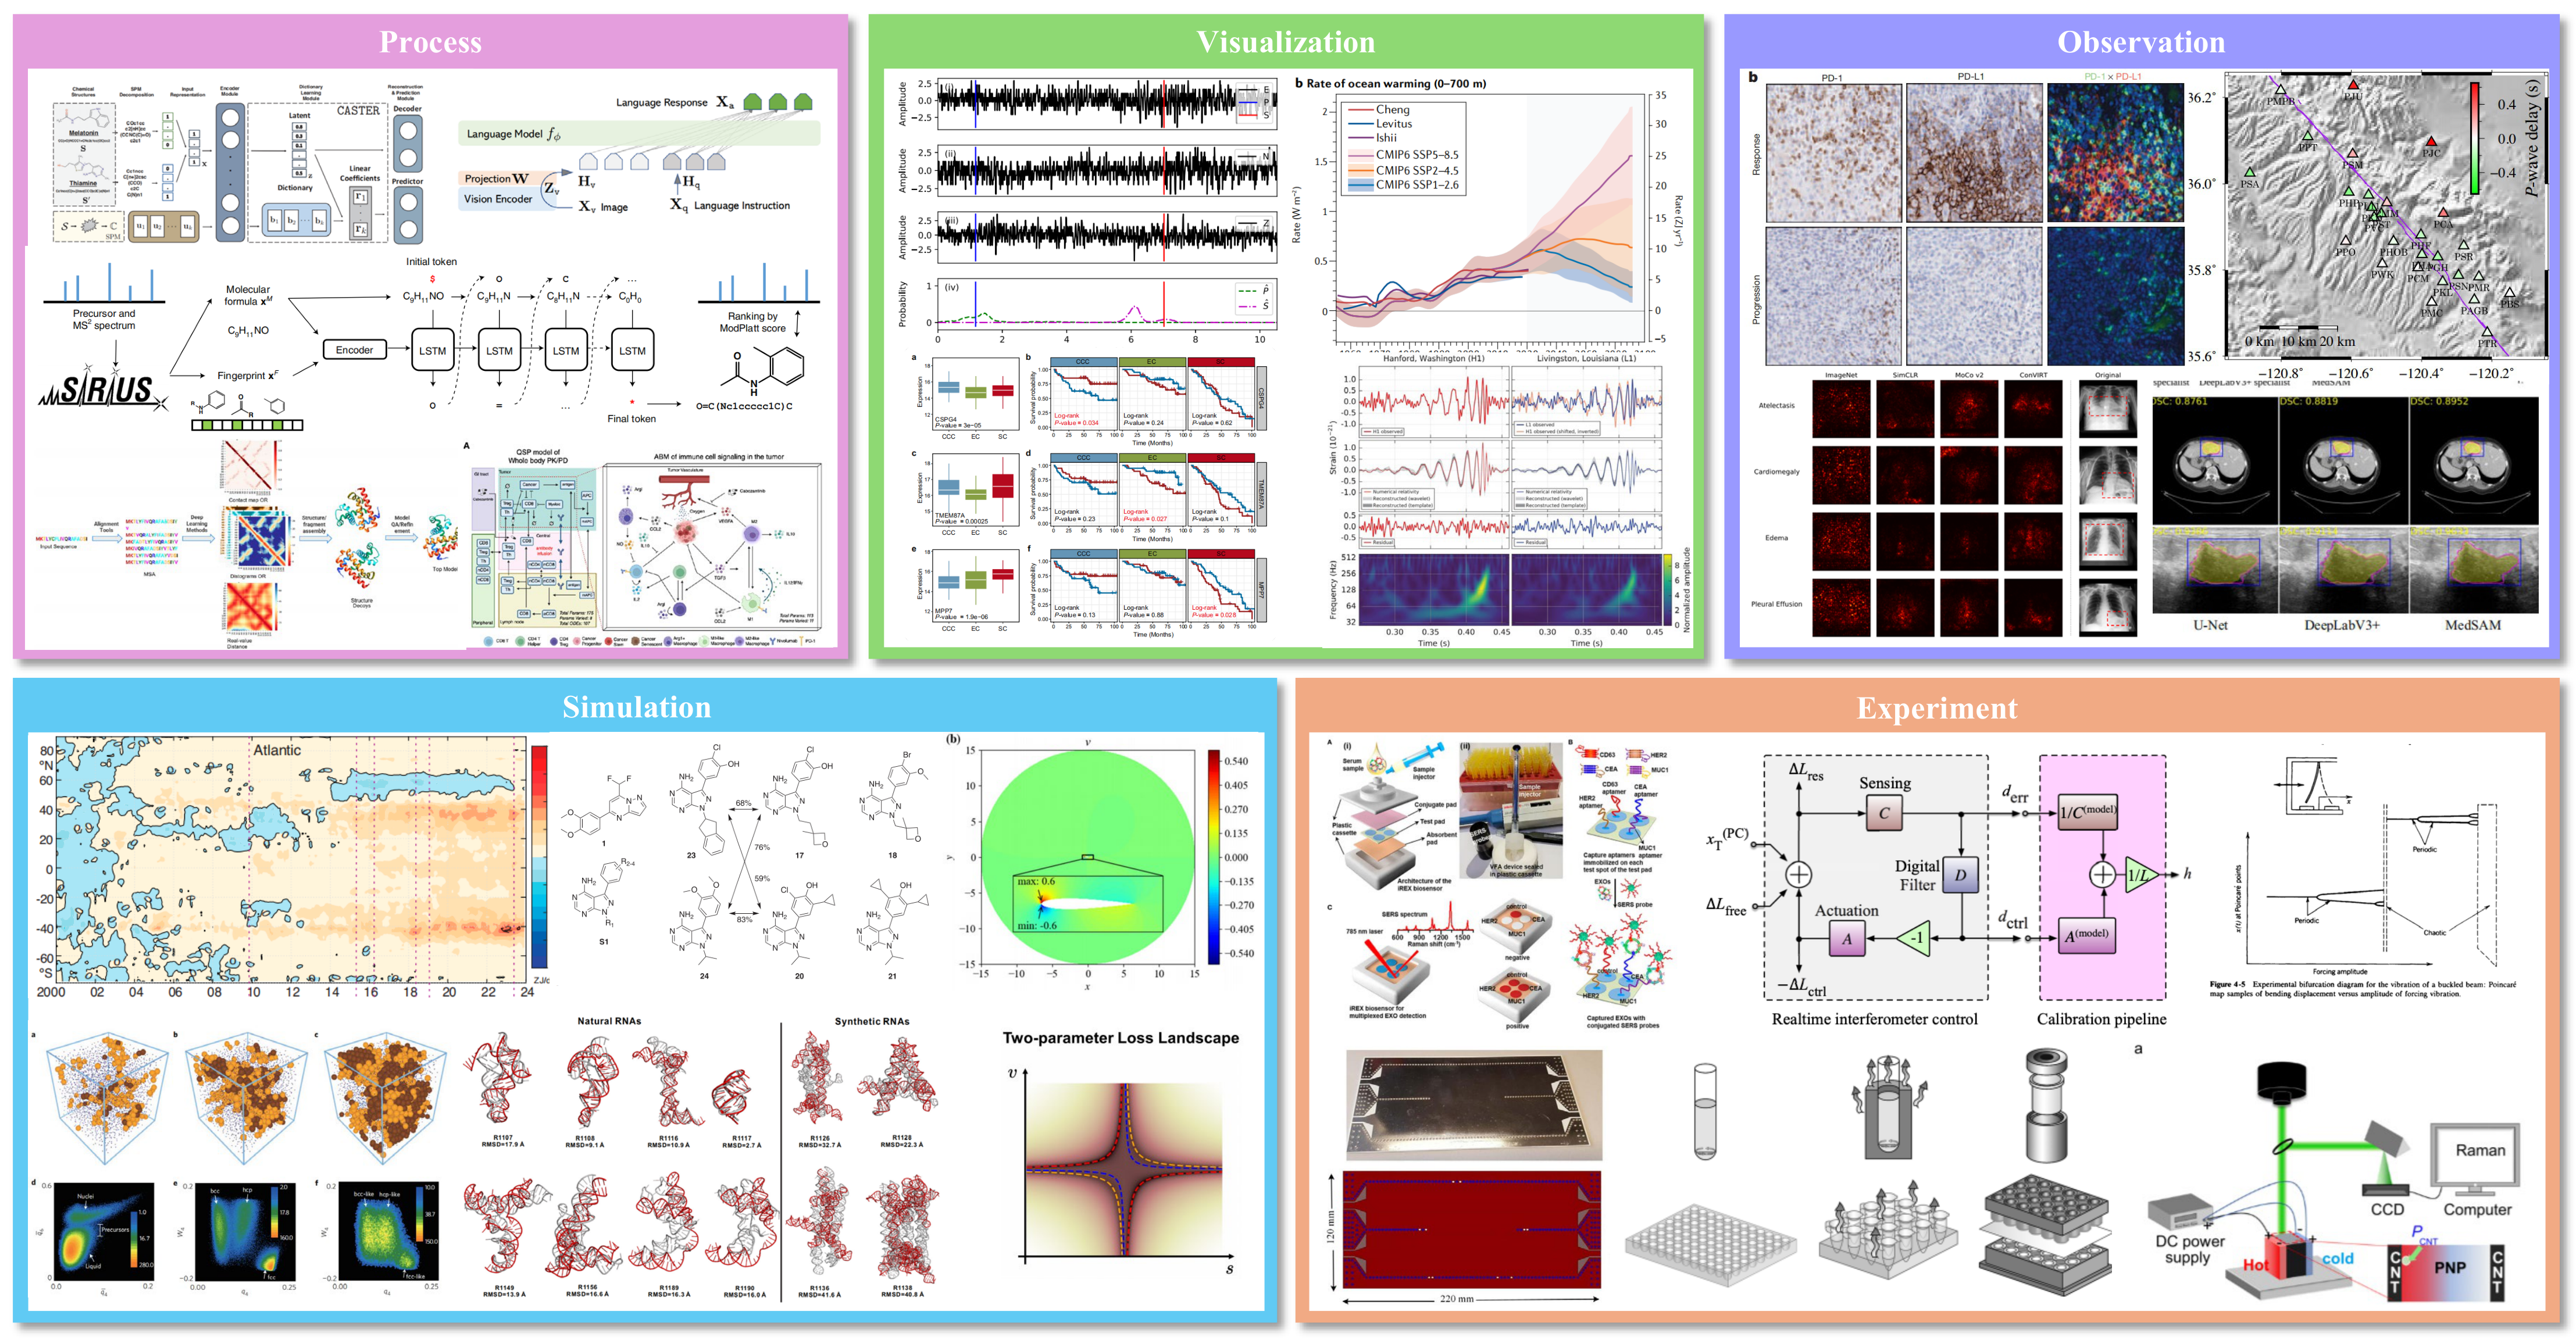
\includegraphics[width=16cm]{paper/imgs/mm_case1.png}}
\caption{\textbf{Scientific Experimental Reasoning Modalities}: Examples of process, visualization, observation, simulation, and experiment images used as multi-modal evidence.}
\label{fig: image_case1}
% \vspace{-2em}
\end{figure}

Scientific Experimental Reasoning evaluates the ability of multimodal LLMs to interpret experimental observations, integrate heterogeneous scientific evidence, and refine testable hypotheses. As illustrated in Figure~\ref{fig: image_case1}, the visual inputs span five representative modalities in scientific practice—process diagrams, data visualizations, natural observations, numerical simulations, and laboratory experiments—reflecting the diversity of multimodal information that underpins real-world scientific inquiry.

\begin{figure}[ht]
% \vspace{-0.5em}
\centerline
{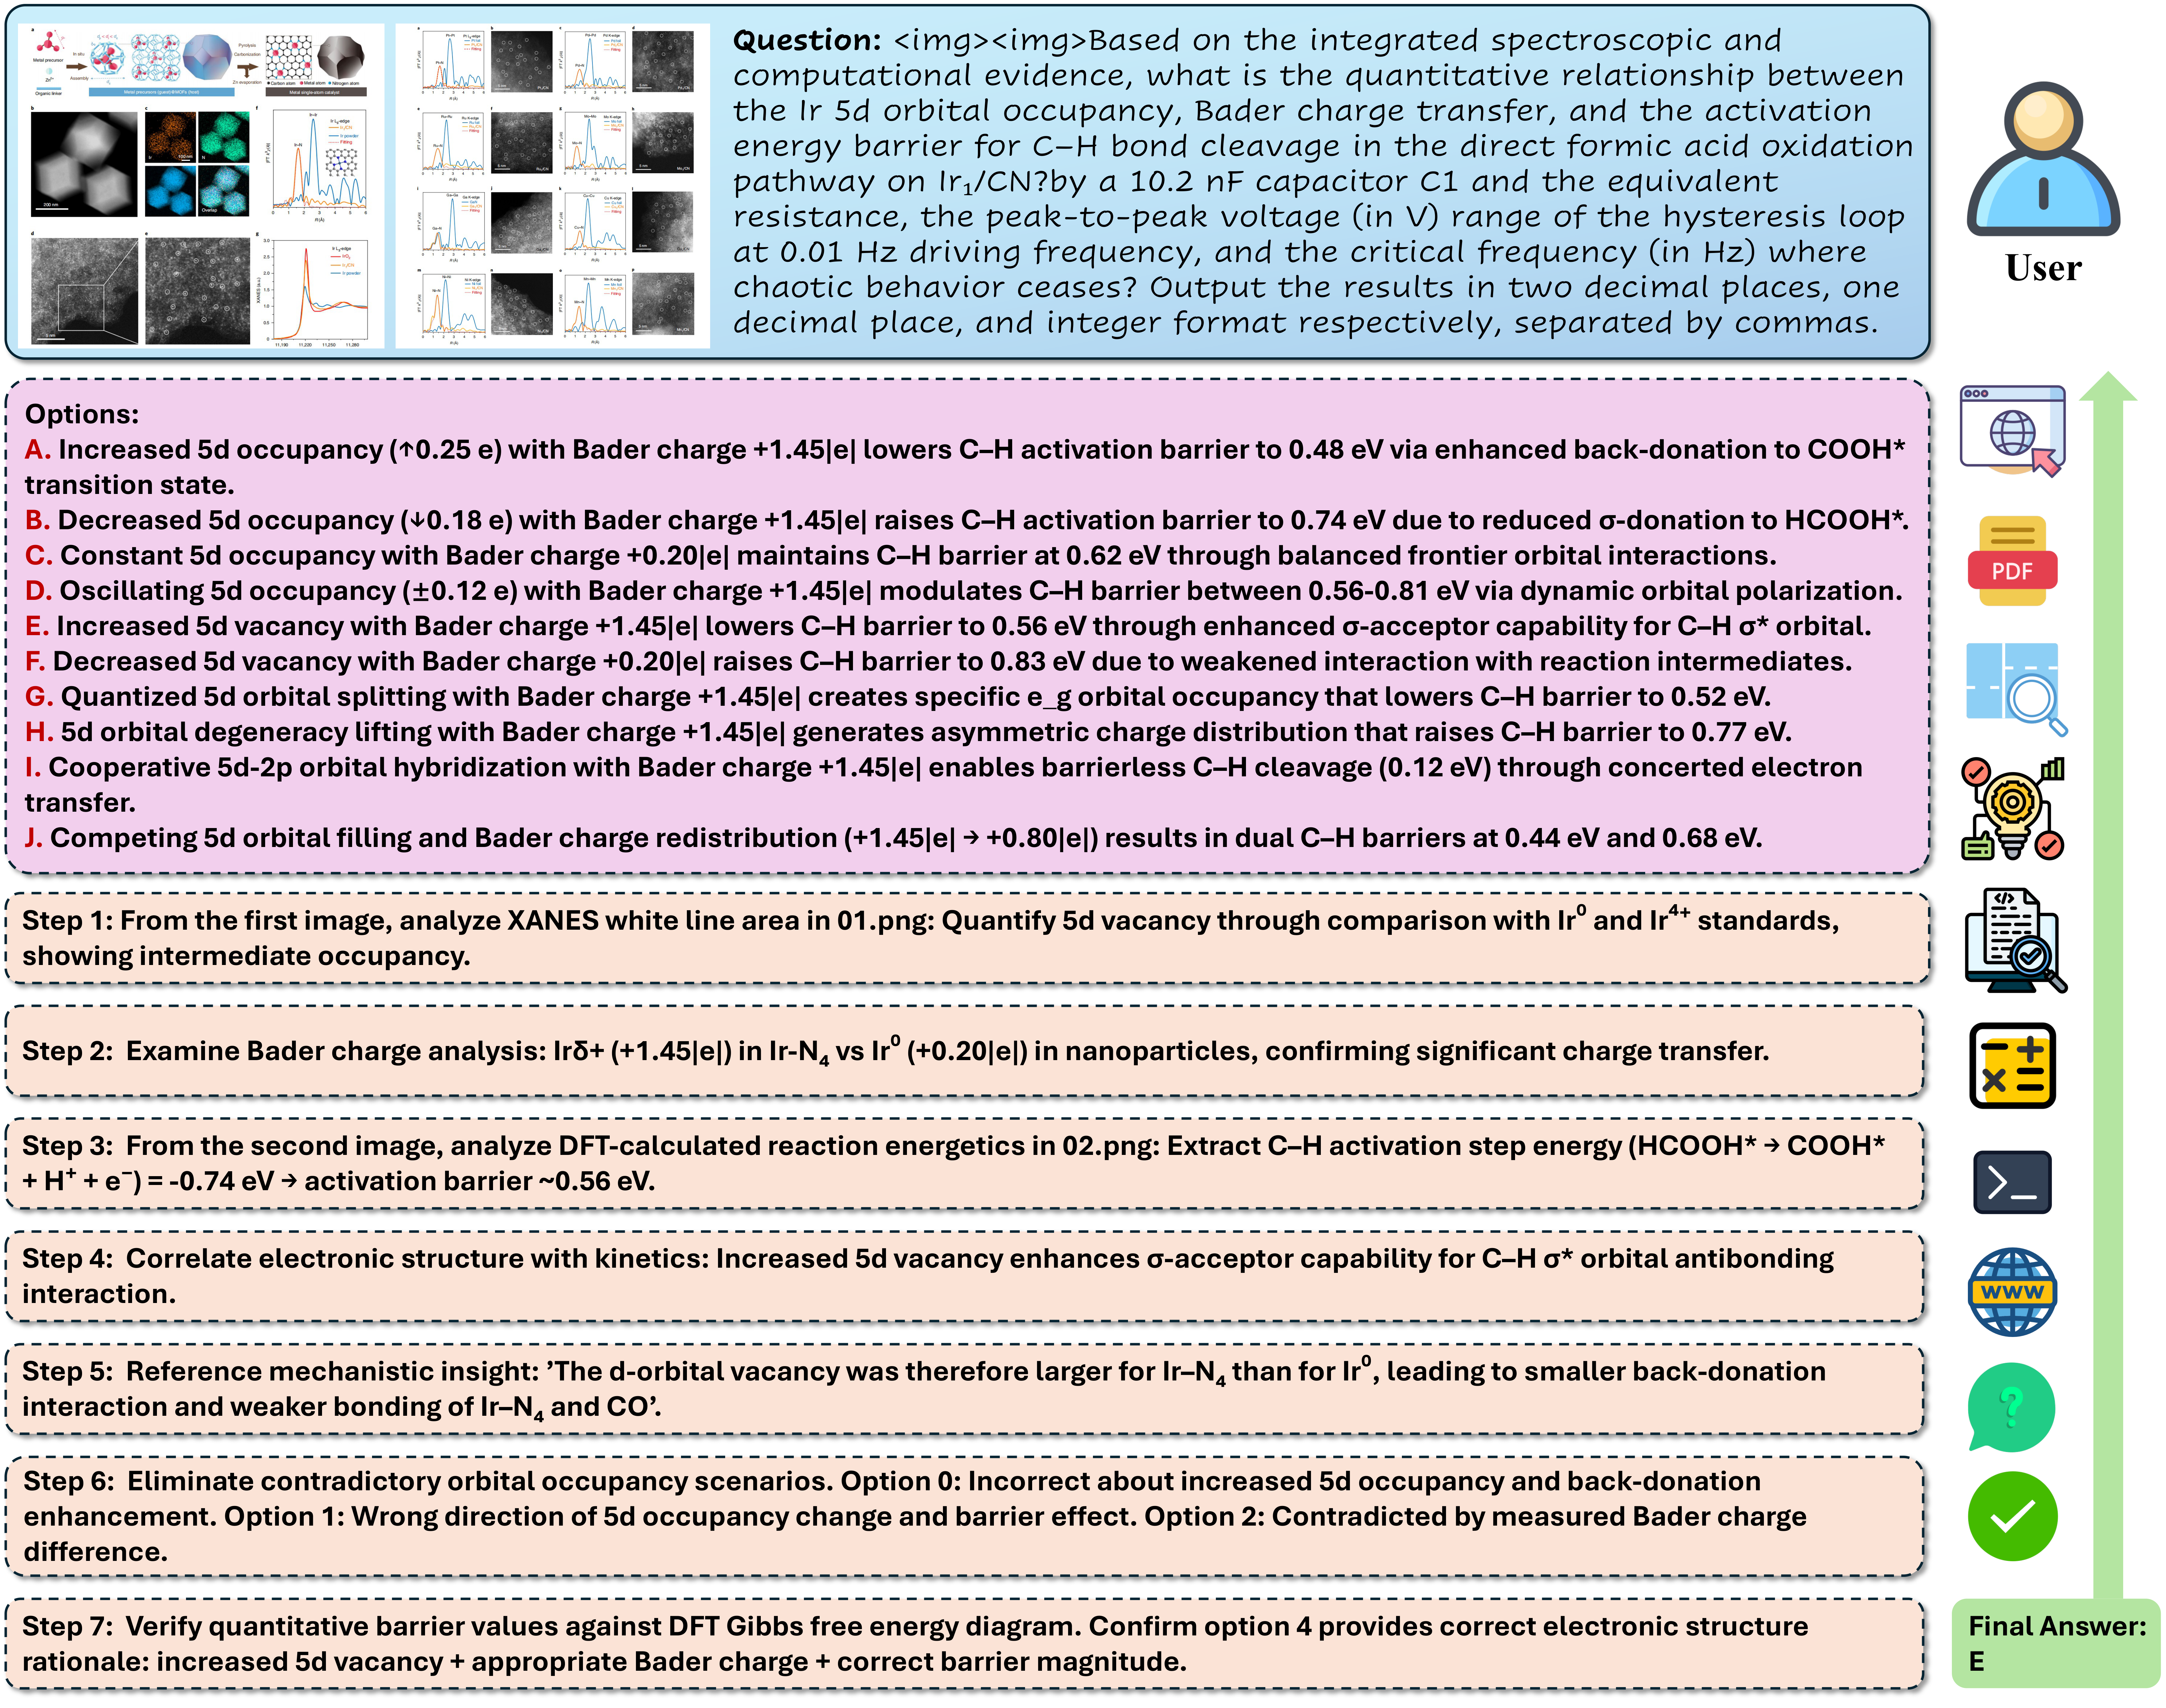
\includegraphics[width=16cm]{paper/imgs/mm_case_1.png}}
\caption{\textbf{Scientific Experimental Reasoning Case}: Multi-image question requiring cross-modal synthesis and step-wise reasoning.}
\label{fig: mm_case1}
% \vspace{-2em}
\end{figure}

In this task, models are provided with several images accompanied by a question and must select the correct answer from at least ten candidates (Figure~\ref{fig: mm_case1}). Solving these problems requires multi-step inferential reasoning: identifying relevant variables, synthesizing multimodal cues, evaluating competing hypotheses, and ultimately validating consistency across the provided evidence. We therefore evaluate model performance using both Multi-choice Accuracy and Reasoning Validity, the latter assessing whether the model’s explanation follows logically from the scientific evidence.

\begin{figure}[ht]
% \vspace{-0.5em}
\centerline
{\includegraphics[width=16cm]{paper/imgs/mcq_metric.png}}
\caption{\textbf{Scientific Experimental Reasoning Evaluation}: Multi-Choice Accuracy (MCA) and Reasoning Validity (RV) across models on multimodal tasks.}
\label{fig: mm_results}
% \vspace{-2em}
\end{figure}

\textbf{Reasoning validity often exceeds answer accuracy.}
As shown in Figure~\ref{fig: mm_results}, closed-source LLMs generally outperform open-source counterparts on both metrics, with the best closed-source models achieving higher MCA (e.g., up to 41.9) and RV (e.g., up to 57.1) than the best open-source models (MCA 37.8, RV 50.5). However, several open-source models remain competitive with or exceed some closed-source systems in specific metrics (e.g., Qwen3-VL-235B-A22B RV 50.5 > GPT-4o RV 45.4), indicating nontrivial overlap. Most models score higher in Reasoning Validity than in Multi-choice Accuracy, suggesting that even when the final choice is incorrect, explanations often preserve partial logical coherence. Variance is moderate—particularly among closed-source models—while only a few models (e.g., Intern-S1-mini) show noticeably lower performance, pointing to the importance of scale for robust multimodal scientific reasoning.


\begin{figure}[ht]
% \vspace{-0.5em}
\centerline
{\includegraphics[width=16cm]{paper/imgs/mcp_task_metric.png}}
\caption{\textbf{Scientific Experimental Reasoning Performance by Type and Discipline}: Breakdown across reasoning paradigms (signal, attribute, comparative, causal) and 10 scientific domains.}
\label{fig: mm_tasks_subjects}
% \vspace{-2em}
\end{figure}

\textbf{Comparative reasoning is the most challenging across domains.}
To further dissect these capabilities, we analyze performance across reasoning types and disciplinary domains (Figure~\ref{fig: mm_tasks_subjects}).
From the perspective of reasoning categories, including signal perception, attribute understanding, comparative reasoning, and causal reasoning, LLMs perform consistently well in causal reasoning and perceptual recognition. In contrast, comparative reasoning emerges as a persistent weakness. This indicates that models struggle when required to contrast subtle quantitative or qualitative differences, a cognitive operation fundamental to scientific evaluation and hypothesis discrimination.
When examining performance across 10 scientific disciplines, an intriguing pattern emerges. Models achieve their highest accuracy in astronomy, followed by chemistry, energy science, and neuroscience. These domains often feature structured visual patterns or canonical experimental setups, which may align well with LLMs’ prior training data. Conversely, performance declines substantially in materials science, life sciences, and Earth sciences, where visual cues are more heterogeneous, context-dependent, or experimentally nuanced. This divergence suggests that domain-specific complexity and representation diversity strongly influence multimodal reasoning performance.

Overall, these findings reveal that while current LLMs demonstrate encouraging abilities in integrating scientific evidence and conducting basic causal analyses, they still fall short in tasks requiring precise discrimination, cross-sample comparison, and nuanced interpretation of domain-specific observations. The relatively narrow performance gap among leading models underscores that scale alone is insufficient; advancing scientific experimental reasoning will require improved multimodal grounding, finer-grained visual understanding, and training paradigms explicitly aligned with scientific inquiry.
